\documentclass{IEEEtran}
\usepackage[english]{babel}
%\usepackage{subcaption}
%\usepackage{comment}
\usepackage{hyperref}
\usepackage{graphicx}
\usepackage{amsmath}
%\usepackage{authblk}
\graphicspath{{images/}}
\usepackage{geometry}
 \geometry{
 a4paper,
 total={170mm,257mm},
 left=15mm,
 top=15mm,
 }
\title{Path planning for Aerial Robots}
\author{
\begin{tabular}[t]{c@{\extracolsep{8em}}c} 
Eashwar Sathyamurthy  \hspace{2in} Akwasi A Obeng \\
Robotics Engineer \hspace{2in} Robotics Engineer \\ 
A. James Clark School of Engineering \hspace{1in} A. James Clark School of Engineering \\
University of Maryland \hspace{2in} University of Maryland \\
College Park, USA \hspace{2in} College Park, USA \\
eashwar@umd.edu \hspace{2in} obenga01@umd.edu
\end{tabular}
}

\begin{document}
\maketitle
\begin{abstract}
In recent times, increase in the usage of automobiles is causing difficulty in transporting goods between two places. As a result, aerial navigation of transporting goods through drones is gaining popularity due to reduced traffic and its ability to reach goal faster. But, aerial navigation also has difficulties such as avoiding collision with tall buildings, changing path to avoid dynamic obstacles etc. Due to these difficulties present, path planning of drones becomes crucial. Hence, there is a need to develop a path planning algorithm which finds the shortest path to reach the goal whilst avoiding static and dynamic obstacles. In this report, we implemented sampling based path planning algorithms to manuever the drone in both static and dynamic environment.
\end{abstract}
\section{\textbf{Introduction}}
Drones in recent times are being used for surveillance in military and for transportation purposes. Mostly recently, drone was used to transplant kidney. Hence, with the commercialization of drones it is important to use a path planning algorithm which can make the drone manuever when faced with random obstacle. 
\begin{figure}[h]
    \centering
    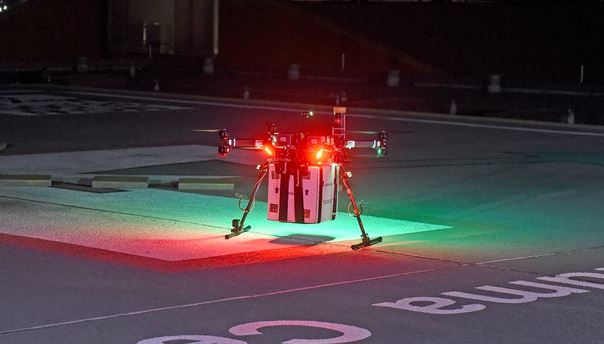
\includegraphics[width=7cm]{kidney}
    \caption{Drone delivering kidney}
    \label{fig:Drone delivering kidney}
\end{figure}
\newline
This report provides detailed implementation RRT and RRT* sampling based algorithms both in 2D and 3D and provides comparison. Furthermore, the algorithm has been developed to avoid dynamic obstacles. This report provides the simulation results of both static and dynamic obstacle avoidance in 3D.
\section{\textbf{Plan of Action}}
\subsection{\textbf{Designing the environment}} 
The first plan of action would be to create an environment for the drone to spawn. The environment should contain obstacles which should be avoided by the drone. The environment is designed both in 3D and 2D (projection of 3D). Initially, it is better to assume the environment to be static. Then after successfully implementing the path planning algorithm in static environment, dynamic obstacles are introduced and the algorithm is changed accordingly. The figure below shows the environment in 2D as well as in 3D.
\begin{figure}[h]
    \centering
    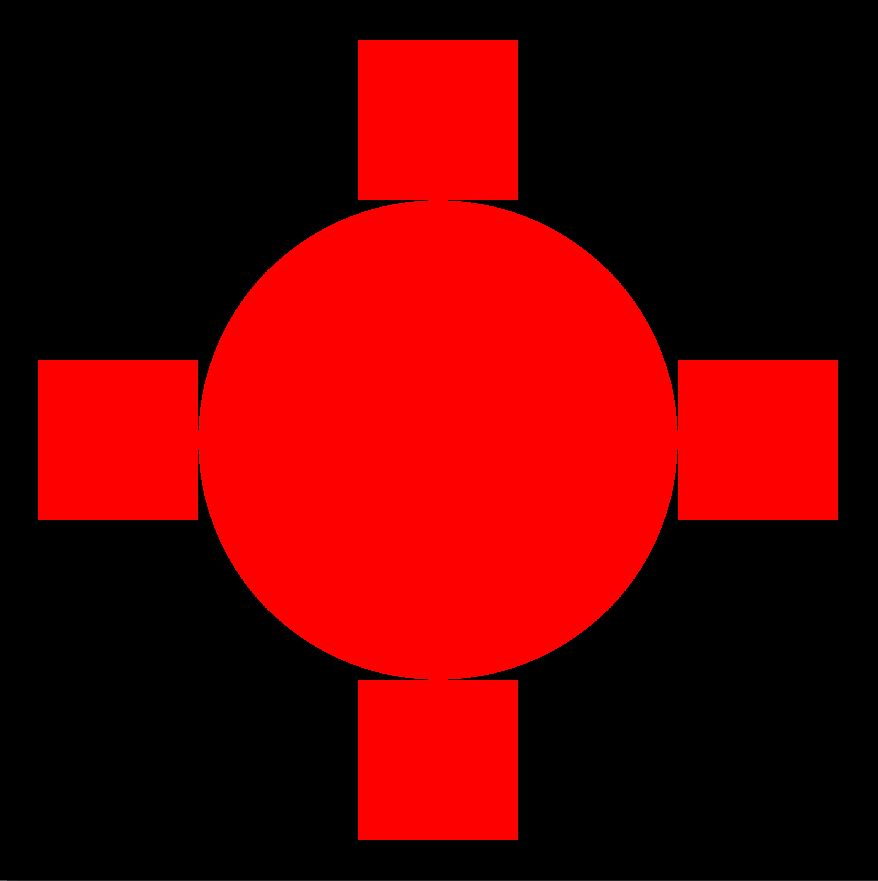
\includegraphics[width=6cm]{2dpygame}
    \caption{2D environment created using pygame}
    \label{fig:2D environment created using pygame}
\end{figure}
\begin{figure}[h]
    \centering
    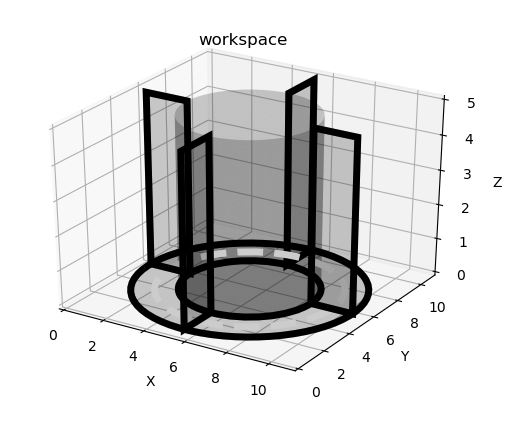
\includegraphics[width=9.5cm]{3dmatplotlib}
    \caption{3D environment created in matplotlib side view}
    \label{fig:3D environment created in matplotlib}
\end{figure}
\newline
This is he environment we created in ROS to spawn the drone.
\newpage
\begin{figure}[h]
    \centering
    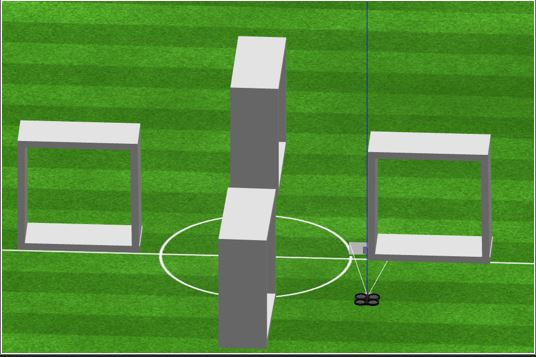
\includegraphics[width=8cm]{gazebo}
    \caption{3D environment created in matplotlib side view}
    \label{fig:3D environment created in matplotlib}
\end{figure}
\subsection{\textbf{Choosing the Path planning algorithm:}}
For this project, the path planning method chosen is RRT and RRT*. Both sampling based algorithms are implemented. First, we need to implement RRT and get a working version on both 2D and 3D environment. Then, we can convert it to RRT* by rewiring. Once we get both RRT and RRT* working for static environment, we can modify the algorithm which can deal with dynamic obstacles.

\subsection{\textbf{Implementing the Path planning algorithm:}}
After choosing the path planning algorithm, it is always important to select a suitable to visualization software to lucidly showcase the nodes exploration and path generation. Hence, the algorithm is implemented on python which provides great visualization tools both for 2D and 3D. For 2D, Pygame library was used. Since, we are dealing with aerial navigation, we were needed to show the nodes exploration happening in 3D so that we can clearly visualize the drone path and also elevation and depression of drone along Z-axis. So, we implemented the algorithm on 3D using matplotlib which enables 3D plots.
\section{\textbf{Path planning method}} 
The path planning method which we choose for the drone mainly depends on the environment and type of obstacles present in the environment. So, before choosing the path planning method, it is important to get familiarize with the obstacle space of the environment. By examining the obstacle space, we can choose which path planning method to use. 

\subsection{\textbf{Types of Obstacles}:}There are two types of obstacles. They are
\begin{enumerate}
\item \textbf{Static obstacles}: These obstacles does not move with respect to time. So, the obstacle space does not change with the passage of time. In an environment consisting of static obstacles, the generation of collision free optimal path happens only once.
\item \textbf{Dynamic obstacles}: These obstacles move with respect to time. So, the obstacle space constantly keep changing with the passage of time.  In an environment consisting of dynamic obstacles, the collision free optimal path changes continuously as dynamic obstacles can come in the way of the path. Thus, the optimal path changes. \\
\end{enumerate} 
As we now have knowledge regarding the types of obstacles, we can develop an approach for path planning. The following approach is followed for path planning:
\begin{enumerate}
\item  \textbf{Graph generation}: The first step of any path planning method is to generate a probabilistic graph of the environment. In order to generate a map, we use RRT graph generation algorithm. The RRT algorithm also takes into account the differential constraints of the drone.\\

\item \textbf{RRT (Rapidly Exploring Random Trees)}: In RRT, the map is explored with the help of trees beginning from the start configuration. Each node of the tree is randomly generated and connected to the end of the tree if the node generated is not in the obstacle space. If the node generated is in the obstacle space, the nearest edge point which is outside of the obstacle is selected.
\begin{figure}[h]
    \centering
    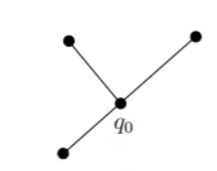
\includegraphics[width=3cm]{RRT1}
    \caption{RRT}
    \label{fig:RRT}
\end{figure}

\begin{figure}[h]
    \centering
    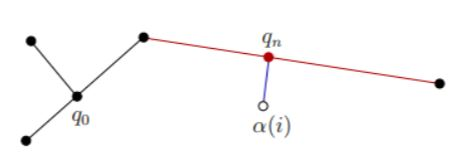
\includegraphics[width=6cm]{RRT2}
    \caption{Connecting the tree to nearest edge point}
    \label{fig:RRT}
\end{figure}
\begin{figure}[h]
    \centering
    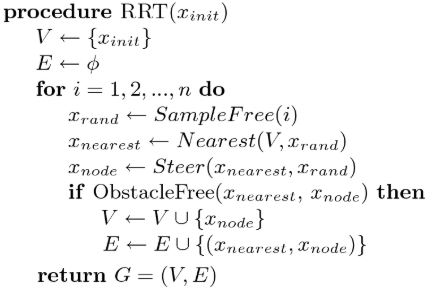
\includegraphics[width=8cm]{pRRT}
    \caption{RRT pseudo code}
    \label{fig:RRT}
\end{figure}
\item \textbf{RRT*}
RRT*is just the extension of RRT but more computationally expensive. RRT* generated more optimized path than RRT. The only difference between RRT and RRT* is that after joining the random node to the point there is a process called \textbf{rewiring} which takes place. In rewiring, all the nodes, surrounding the newly added node is checked for better possible parent which results in minimum cost-to-tome. The rewiring process occurs to the neighboring nodes which are at a threshold distance from the newly added node. The rewiring process makes the path optimal. But as the rewiring process is repeated for all the newly added node, RRT* becomes more computationally expensive than RRT. The main effect of rewiring is that it makes the nodes exploration process spread in the outward direction from the start location in a straight line. This results in getting the optimal path. The figure below shows the comparison of nodes exploration between RRT and RRT*.

\begin{figure}[h]
    \centering
    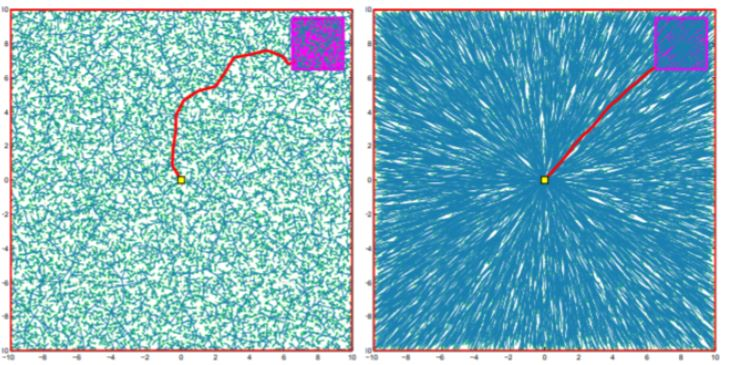
\includegraphics[width=8cm]{pRRT2}
    \caption{RRT  \hspace{1.8in}RRT*}
    \label{fig:RRT}
\end{figure}
The pseudo code for RRT* is given below:
\begin{figure}[h]
    \centering
    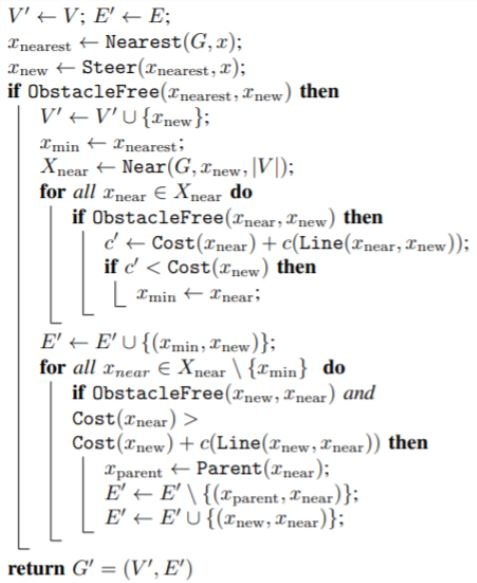
\includegraphics[width=8.5cm]{pRRT1}
    \caption{RRT* pseudo code}
    \label{fig:RRT}
\end{figure}

\item {Smoothing the Solution Path:}
After getting the solution path, in order to avoid steep edges smoothing is done. Smoothing avoids sharp edges which makes it easy for the drone to follow the solution path. We used gradient descent algorithm to smoothen the solution path. Gradient descent algorithm tries to minimize the error between the solution path and smooth path till the error converges to a threshold value. The following is the equation where the smoothing happens.
\boldmath	
\begin{equation}
y_i = y_i + \alpha(x_i - y_i) + \beta(y_{i+1} + y_{i-1} - 2*y_i)
\end{equation}
\unboldmath
\begin{center}
where $x_i$ is the $i^{th}$ solution coordinate \\
        $y_i$ is the  $i^{th}$ smoothened coordinate \\
	$y_{i-1}$ is the  $(i-1)^{th}$ smoothened coordinate \\
	$y_{i+1}$ is the  $(i+1)^{th}$ smoothened coordinate \\
	$\alpha$ is the smoothing coefficient which controls the degree of smoothing \\
	$\beta$ is the weight given to each solution node in the solution path \\
\end{center}
By tuning the $\alpha$ and $\beta$ parameters we can control the smoothing process.
\end{enumerate}
\section{ \textbf{Path planning for Dynamic obstacles:}}
For dynamic environment, we have created moving drones as dynamic obstacles. We have modified RRT and RRT* algorithm to make it work in a dynamic environment. For dynamic environment, we are constantly keeping track the distance of the obstacles from the drone path. If an obstacle obstructs the generated drone solution path and also very close to the drone, process of replanning the path takes place. In replanning, we basically implement the RRT/RRT* algorithm, from the current position of the drone to the goal position with the updated environment(Obstacle blocking drone's path). Hence, the RRT/RRT* generates new path avoiding the obstacle. This process continues till the drone reaches the goal point.
\section{\textbf{Software and Visualization tool Used}}
\begin{enumerate}
\item Python version 3
\item Python version 2.7
\item Matplotlib
\item Pygame
\end{enumerate}
\section{\textbf{Results}}
\subsection{\textbf{Implementation of RRT and RRT* in 2D environment}}
We first implemented RRT and RRT* in 2D using pygame. The following are the plots obtained:
\begin{figure}[h]
    \centering
    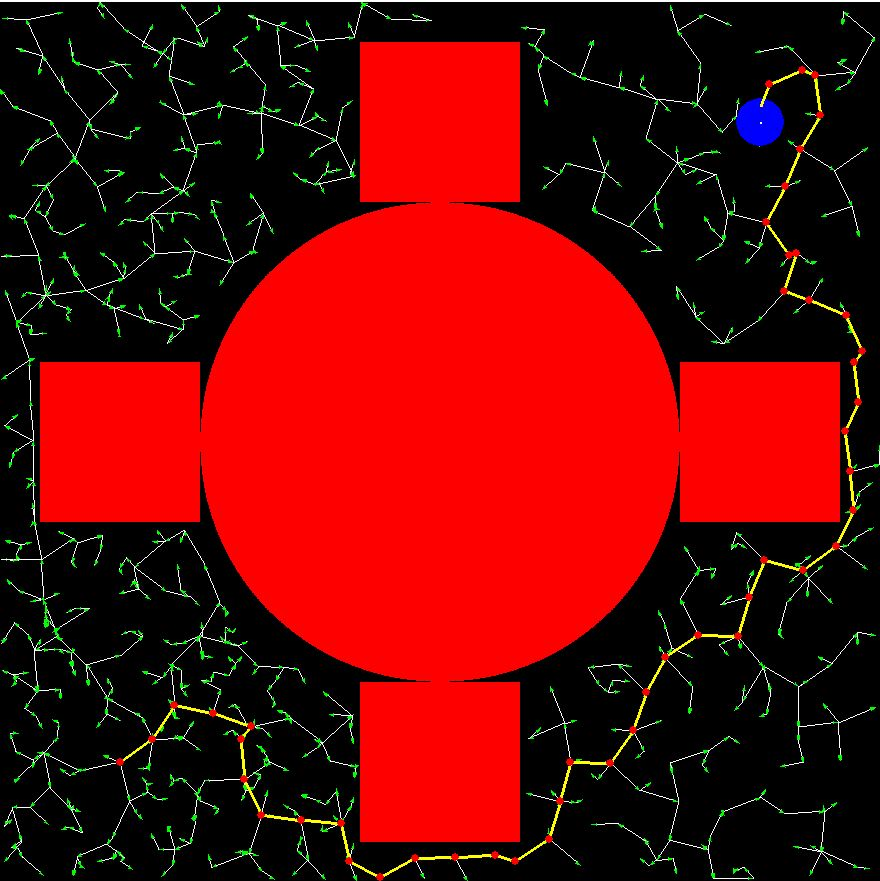
\includegraphics[width=8cm]{rrt2d}
    \caption{RRT implementation in 2D}
    \label{fig:RRT implementation in 2D}
\end{figure}
\newline 
The simulation time for RRT is about 2 seconds. We can clearly see that the path obtained is not optimal but the we get to the solution faster.
\newpage
\begin{figure}[h]
    \centering
    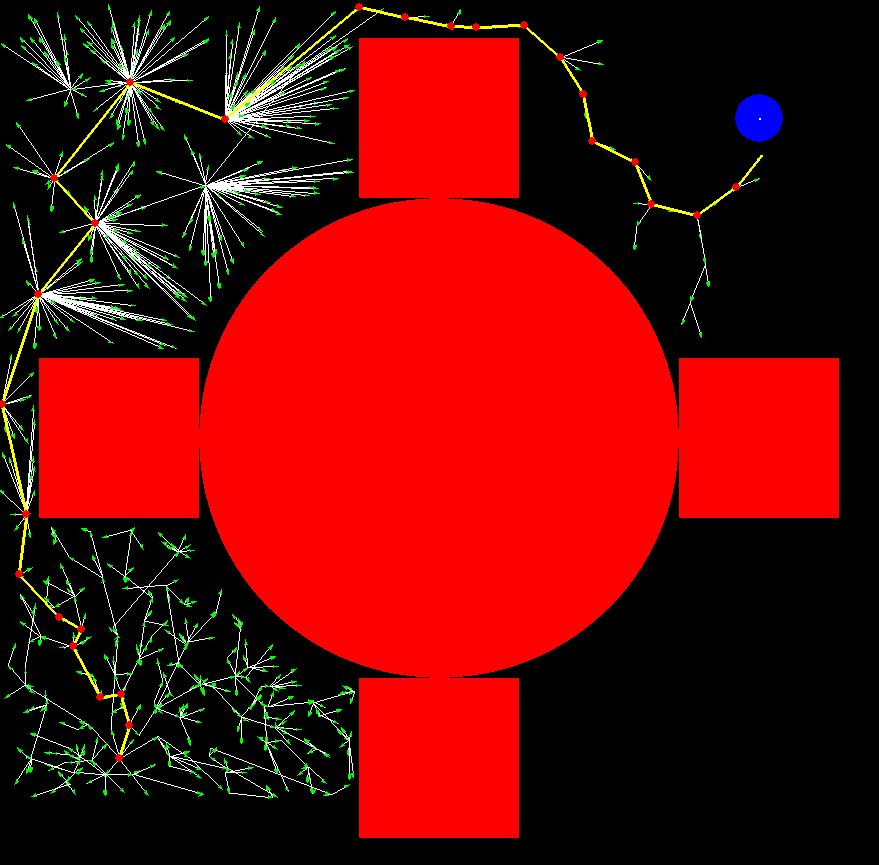
\includegraphics[width=8cm]{rrt2d1}
    \caption{RRT* implementation in 2D}
    \label{fig:RRT* implementation in 2D}
\end{figure} 
The simulation time for RRT* is about 113 seconds. We can clearly see that the path obtained is more optimized than RRT but the time taken to reach the solution is significantly increased. The nodes exploration is directed towards the goal position.

\subsection{\textbf{Implementation of RRT in 3D environment}}
As earlier mentioned, for simulation in 3D matplotlib package was used. The following are the results of RRT and RRT* for a static 3D environment.
\begin{figure}[h]
    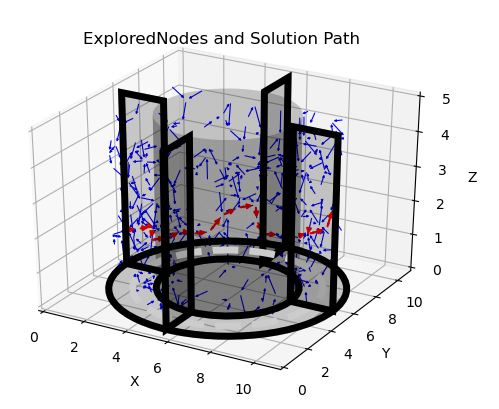
\includegraphics[width=9cm]{rrt3d}
    \caption{RRT implementation in 3D}
    \label{fig:RRT implementation in 3D}
\end{figure} 
\newpage
\begin{figure}[h]
    \centering
    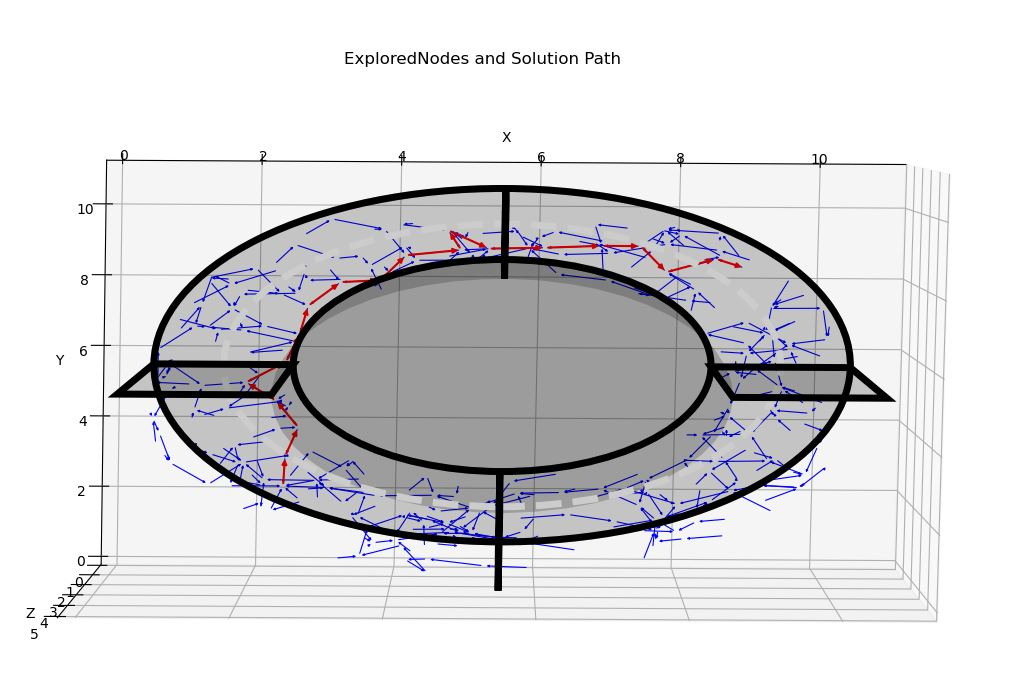
\includegraphics[width=10cm]{rrt3dtop}
    \caption{RRT implementation in 3D top view}
    \label{fig:RRT implementation in 3D top view}
\end{figure}
In addition to this, we have created an animation of drone using matplotlib which follows the solution trajectory.
 \begin{figure}[h]
    \centering
    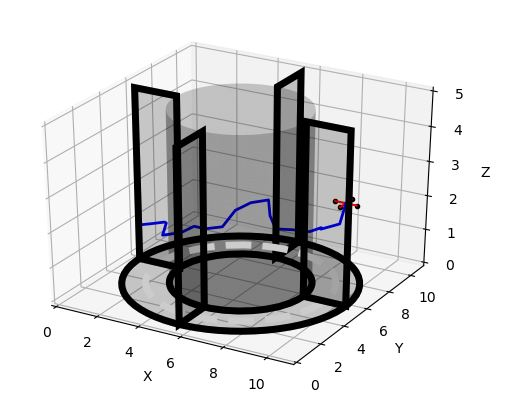
\includegraphics[width=9cm]{rrt3ddrone}
    \caption{RRT implementation drone animation}
    \label{fig:RRT implementation drone animation}
\end{figure}
\newline 
Currently, the path generated by RRT is not smoothened. By implementing the gradient descent algorithm, the solution path is smoothened. The following is the drone trajectory after the path of the drone is smoothened. As RRT generates new path each time, the path shown in the below figures may be little different from the above graphs but difference in the smoothness of the path is clearly seen.
\newpage
\begin{figure}[h]
    \centering
    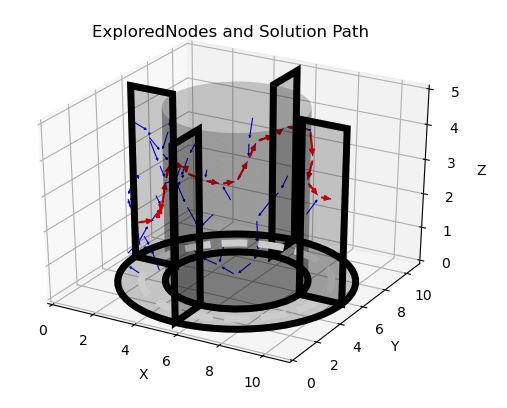
\includegraphics[width=10cm]{rrt3dsmooth}
    \caption{RRT implementation in 3D with smoothing}
    \label{fig:RRT implementation in 3D with smoothing}
\end{figure}
\begin{figure}[h]
    \centering
    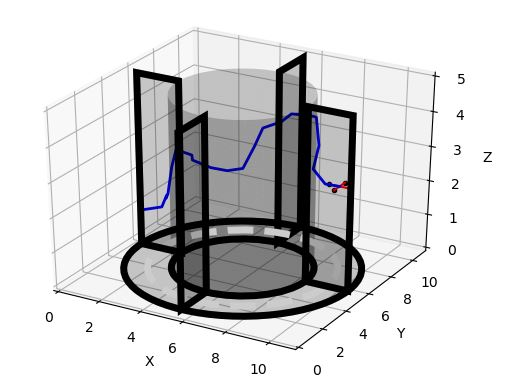
\includegraphics[width=10cm]{rrt3dsmoothdrone}
    \caption{RRT implementation in 3D smooth drone path}
    \label{fig:RRT implementation in 3D smooth drone path}
\end{figure}
\subsection{\textbf{Implementation of RRT* in 3D environment}}
Similar to RRT, we also implemented RRT* algorithm for a static 3D environment. Here are the results:
\begin{figure}[h]
    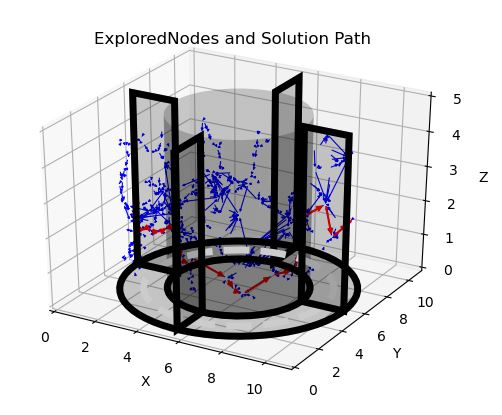
\includegraphics[width=9cm]{rrtstar3d}
    \caption{RRT* implementation in 3D}
    \label{fig:RRT* implementation in 3D}
\end{figure} 
\newpage
\begin{figure}[h]
    \centering
    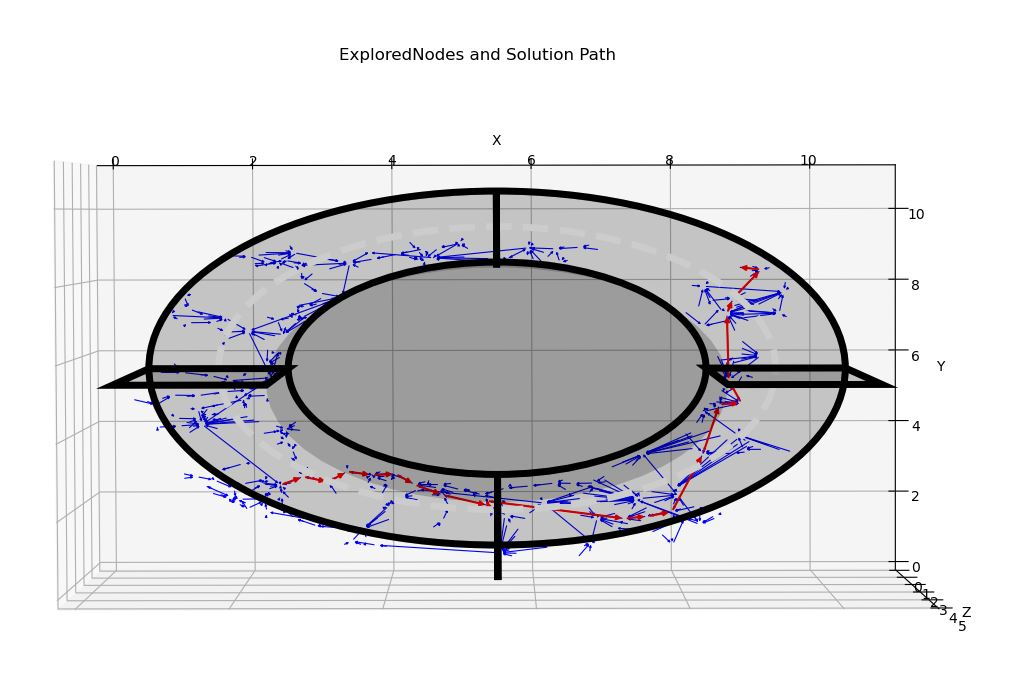
\includegraphics[width=10cm]{rrtstar3dtop}
    \caption{RRT* implementation in 3D top view}
    \label{fig:RRT* implementation in 3D top view}
\end{figure}
\newpage
 \begin{figure}[h]
    \centering
    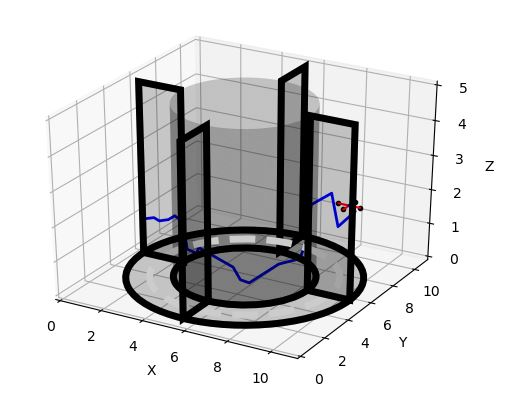
\includegraphics[width=8cm]{rrtstar3ddrone}
    \caption{RRT* implementation drone animation}
    \label{fig:RRT* implementation drone animation}
\end{figure}
After performing the smoothing, the following are the results:
\newpage
\begin{figure}[h]
    \centering
    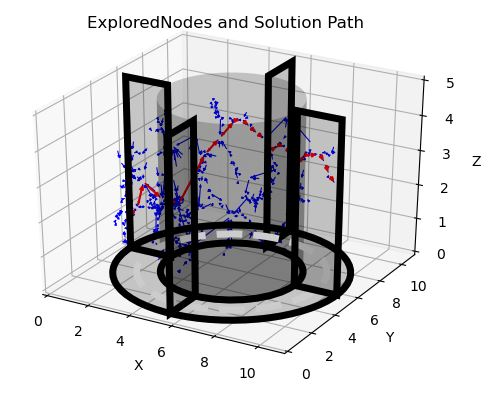
\includegraphics[width=8cm]{rrt3dstarsmooth}
    \caption{RRT* implementation in 3D with smoothing}
    \label{fig:RRT* implementation in 3D with smoothing}
\end{figure}
\newpage
\begin{figure}[h]
    \centering
    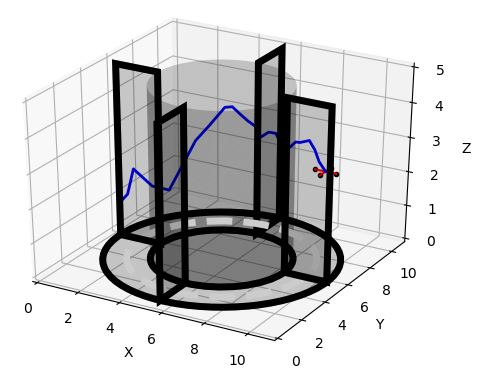
\includegraphics[width=8cm]{rrtstar3dsmoothdrone}
    \caption{RRT* implementation in 3D smooth drone path}
    \label{fig:RRT* implementation in 3D smooth drone path}
\end{figure}
\subsection{\textbf{Dynamic Environment path planning results:}}
We have developed RRT and RRT* algorithms to adapt to dynamic changes in the environment. Below sequence of images explains the pipeline with the output results. The following are the results obtained:
\begin{enumerate}
\item First RRT/RRT* generates the initial solution path considering the initial position of the obstacles(drones).
\begin{figure}[h]
    \centering
    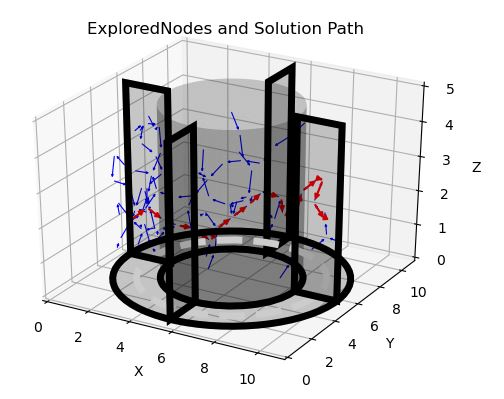
\includegraphics[width=8cm]{s2}
    \caption{Generating initial solution path}
    \label{fig:Generating initial solution path}
\end{figure}
\item The drone animation below shows the drone starting to the follow the initial generated solution path.
\newpage
\begin{figure}[h]
    \centering
    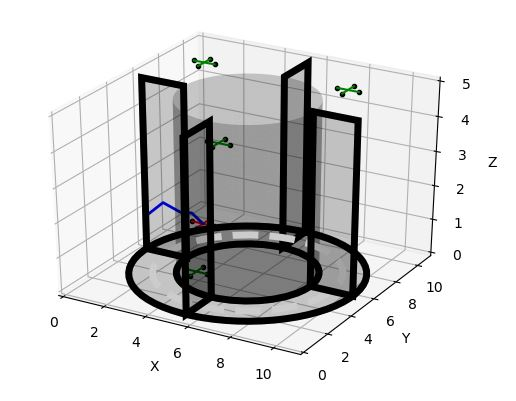
\includegraphics[width=8cm]{s1}
    \caption{Drone following the initial solution path}
    \label{fig:Drone following the initial solution path}
\end{figure}
\item In the above picture, one of the obstacle drone was obstructing as well as close to the drone. Hence, replanning of the path occurs.
\begin{figure}[h]
    \centering
    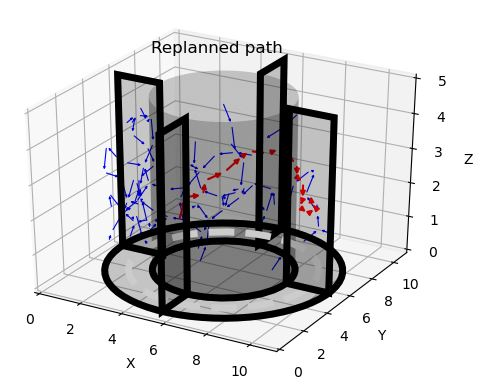
\includegraphics[width=8cm]{replanned}
    \caption{Replanning of drone path from current position}
    \label{fig:Replanning of drone path from current position}
\end{figure}
\item Now the figure below shows the animation of the drone following the replanned path
\begin{figure}[h]
    \centering
    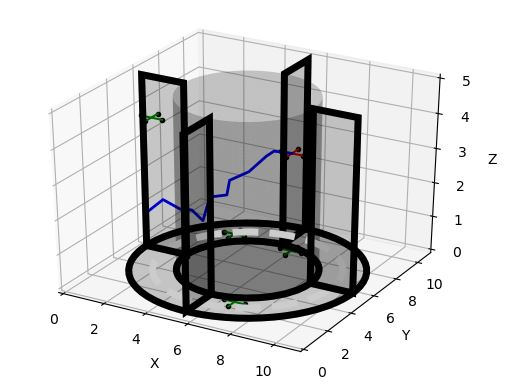
\includegraphics[width=8cm]{replanned1}
    \caption{Drone following replanned path}
    \label{fig:Drone following replanned path}
\end{figure}
\end{enumerate}
\section{\textbf{Goal Achieved:}}
\begin{enumerate}
\item Successfully implemented RRT and RRT* algorithms in 2D in static environment.
\item Successfully created a dynamic obstacle space in 3D.
\item Successfully implemented RRT and RRT* algorithms in static and dynamic environment in 3D.
\item Successfully smoothened the solution path using gradient descent algorithm.
\end{enumerate}
\section{\textbf{Future Scope}}
Our future goal would be to integrate the algorithm with ROS and provide a simulation in gazebo. 
\section{References:}
\section{Team members}
\begin{enumerate}
\item Eashwar Sathyamurthy
\item Akwasi A Obeng
\end{enumerate}
\end{document}
